\documentclass[format=sigconf]{acmart}
\settopmatter{printacmref=false} % Removes citation information below abstract
\renewcommand\footnotetextcopyrightpermission[1]{} % removes footnote with conference information in first column
\usepackage[utf8]{inputenc}
\usepackage{amsmath}

\settopmatter{printacmref=false}

\title{Mathematical model approach for draft picking in basketball}

\author{Lawrence Thanakumar Rajappa}
\affiliation{\institution{IDA Linköping University}}
\email{lawra776@student.liu.se}

\date{December 2020}

\begin{document}
\maketitle
\pagestyle{plain} % Remove ACM page header

\section{Introduction}
Analytics is being used in all fields such as healthcare, manufacturing, banking and etc. for decision-making. Likewise, 
analytics is also playing a major role in Sports industry such as football, baseball, basketball and etc. to predict player's 
next move, injury analysis, position analysis and etc. Sports analytics is being spoken as a concept for many years which 
could be used to improve team performance, as a result, the revenue generation is very much improved for the team. For this 
project, we will mostly focus on basketball. In order to have a good prediction and analysis report, we need to have proper
dataset and most importantly, the data must have most important attributes that could provide insights for a given problem.

There are many ways that the data can be used by the team for various purposes. The kind of data that the team would use includes
average stats of the players, per game stats, and etc. These data can be used to understand a player in terms of strengths and 
weaknesses, emotional stability and etc. These attributes could be used to assess the team's performance. Moreover, there are other 
attributes such as weather conditions, the condition of the field and even psychological factors such as the fans support should be
included along with player's data to determine the team's performance. This document speaks about how the data are being used by
a basketball team to select players using mathematical models.

\section{Aim}
In this project, the aim is to create a draft picking system for a basketball team by using 3 mathematical models namely, model 1 : model
to predict whether a player will stay in the team for five years or not, model 2: model to determine the position of players 
based on their previous experiences and model 3: model to cluster or group players based on previous performances. These models
would facilitate team managers and coaches to select players and make best out of them.

\section{Motivation}
Before the advent of analytics, the selection of players or draft formation was done manually which was a time consuming and huge 
workload. The emergence of analytics and computing resources has paved a new way in recruiting best players based on their previous
performances in a short period of time with minimal workload. However, Sports industry has restricted for the complete adoption of 
analytics into their respective teams because teams spend three-fourth of their revenue for paying salaries to the players
and to cover other expenditures. Hence, the teams cannot afford to invest huge sum of money in technology, data and analytical 
tools  \cite{davenport2014analytics}. This project would remove the above mentioned bottleneck and facilitate the teams to use 
analytical tools with much lower cost and at ease. 

\section{Earlier system}
Earlier to 2005, the data was collected by a person watching the game using either a notepad and pen or black boards with chalks.
This data was prone to human errors. As a result, the analysis carried out on this data and results were misleading.
In 2005, two Isareli scientists, Gal Oz and Miky Tamir, created a system called \textit{SportsVU} (see in figure \ref{fig:SportsVU})
\cite{mccann2012player} \cite{warsaw}. This
system captures the ball movement as well as athletes movement, all these data are combined together for statistial analysis using 
the statistical algorithms that the company has created \cite{warriors}.
Based on the statistial analysis inference, the players were chosen for a team, but this method was manual. Moreover, other data such 
as Rebounds, TurnOver and etc were calculated from this system as well as from manually gathered data.

\begin{figure}[H]
    \centering
    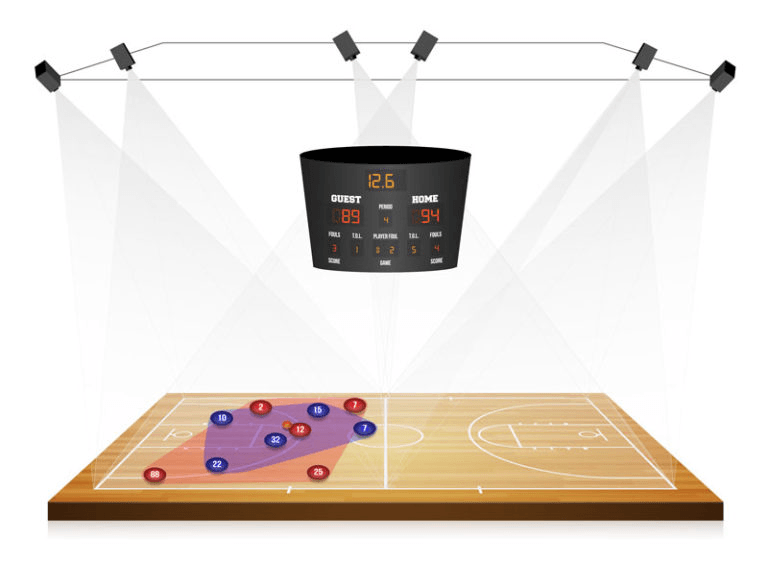
\includegraphics[scale=0.20]{STATS-SportVU-technology.png}
    \caption{SportsVU in basketball court.}
    \label{fig:SportsVU}
\end{figure}

\section{Background}
In this part, some general terms that are relative to the topic are going to be discussed. It is important to understand them for further
reading. 

The terms that will be discussed are:
\begin{itemize}
    \item  Draft picking and its process.
    \item  Machine or mathematical learning.
    \item  Sports Analytics.
\end{itemize}
\subsection{Draft picking and its process}
\bibliographystyle{ACM-Reference-Format}
\bibliography{references}
\end{document}

